\documentclass{article}
\usepackage[utf8]{inputenc}

\title{Midterm}
\author{Muhammed Yasir Fidan }
\date{May 2021}

\usepackage{natbib}
\usepackage{graphicx}

\begin{document}

\maketitle

\section{Report}
Firstly, I use 7 posix named semaphores in my program. I hold my buffer as a shared memory. Empty semaphore and mshare semaphore same as producer comsumer program semaphores that we saw in class. I use empty semaphore in nurse processes. Empty semaphore check there is still empty space in buffer or not. Empty semaphore initilize as buffer size at the beginning. If it become 0 all nurses wait for some vaccinator and citizens use vaccines and make empty spaceses in buffer. Then Nurses can continue to fill buffer. \\
The mshare semaphore again very similar to producer consumer semaphore. I use it to lock whenever I access shared memory. Because I don't want to more than 1 process can access shared memory at the same time. If they can reach at the same time, They can corrupt memory so mshare used for critical section locks. \\
Figure 1 is containe my nurse process code. All process read 1 character from file. I use exclusive lock when reading char because I don't want to 2 process read at the same time. Maybe they can read same character if they read at the same time so when reading I use exclusive lock. After processes read 1 character they use empty semaphore to check there is empty space in buffer or not. If there is empty space processes continue. Then only one process enter mshare semaphore critical region like in producer consumer problem. Kernel choose one of the nurse process and it enter mshara critic area. This is critical area because I access my buffer here. If nurse has a vaccine 1 insertBuffer function add a vaccine 1 to the buffer. If nurse has a vaccine 2 insertBuffer function add a vaccine 2 to the buffer. Then I take how many vaccine 1 and vaccine 2 in my buffer by using numberOfVaccine1 and numberOfVaccine2 functions. Then I use 2 more semaphore here. removeVac and atomicWait. atomicWait used in vaccinators. All vaccinators wait for there is at least 1 vaccine 1 and 1 vaccine 2 in buffer. In nurse, here I check there is currently enough vaccines for a new vaccinator to run by using removeVac and atomic. If there is both 1 and 2 vaccine in buffer now a vaccinator that wait in atomicWait semaphore now can continue. After that nurse relase mshare lock. Now kernel continue with same nurse or other nurses same process again until nurses reach end of file.
\begin{figure}[h!]
\centering
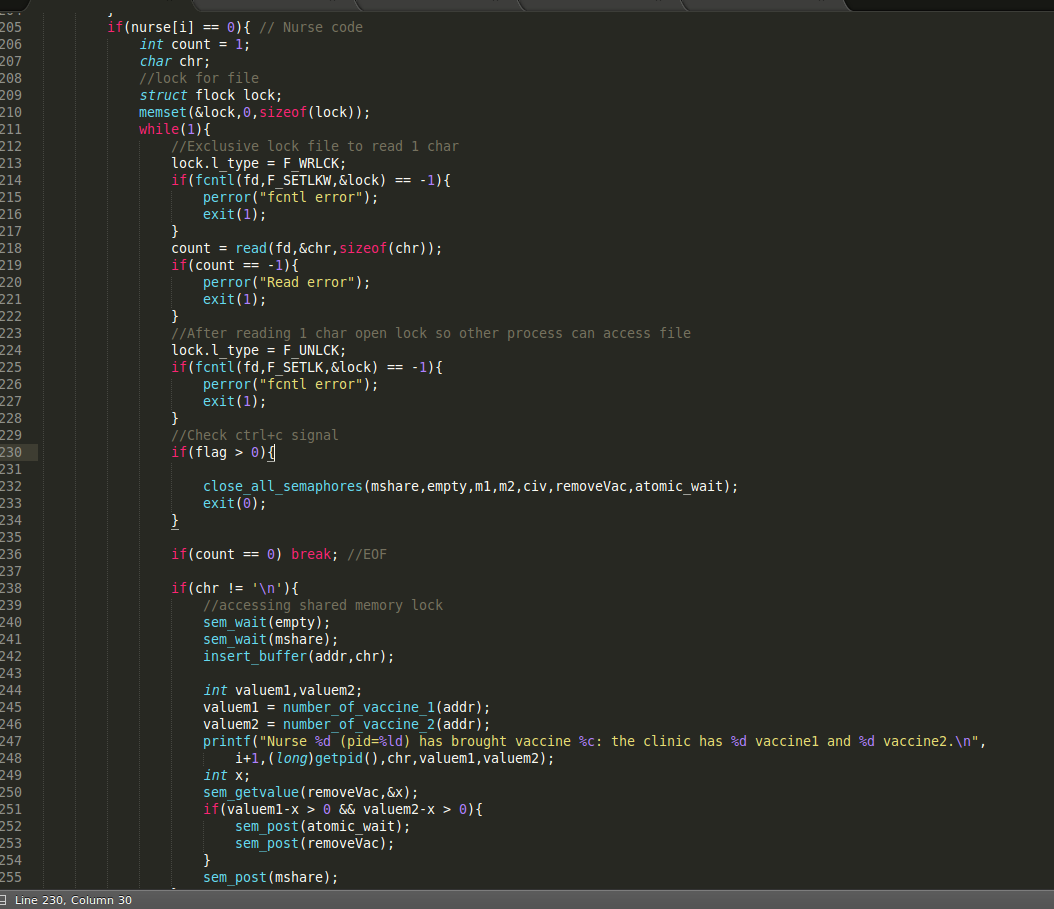
\includegraphics[scale=0.35]{nurse.png}
\caption{The Nurse process code}
\label{fig:nurse}
\end{figure}
\newpage
Figure 2 containe my vaccinator process code. In vaccinator first I check in critical section there is enough vaccinator for my program already or not. Because file will containe 2*t*c character so vaccinators work for t*c times total. So I check it at the begginning of vaccinator code. If vaccinator already executed for t*c times it means all citizens already finished. So vaccinators stop in if statement and they start exit too after closing all semaphores. \\
But this is the case for exit of vaccinators. If there are still citizens must invite, they continue simultaniously and stuck in atomicWait semaphore. They wait here for at least there will be 1 vaccine1 and 1 vaccine2 in buffer. So I explained in above nurses increment this semaphore when ever there is enough vaccines for a vaccinator. So kernel choose one of them and this vaccinator can continue and others wait for more vaccines. Then one of the vaccinator enter critical region because I modify shared memory here. First Vaccinator decrease removeVac semaphore and call remove1and2 function. This function removes 1 vaccine1 and 1 vaccine2 in buffer. Then I use my fifth semaphore civ. Vaccinator post civ semaphore so 1 of the citizen process awakened. Then I construct a fifo between this vaccinator and awakened citizen because I need citizen pid. After reading citizen pid from fifo, Vaccinator print invite message something in pdf. After that I use my second shared memory. I use this memory to hold which vaccinator invete how many people information. So I increment 1 for this vaccinator because he/she invite a citizen. Then I use my last 2 semaphore those are m1 and m2. I used this semaphores for ensure first write invite message than citizen vaccinated message. After that Vaccinator release lock and increment empty semaphore 2 times. Because he/she use 2 vaccine. \\




\begin{figure}[h!]
\centering
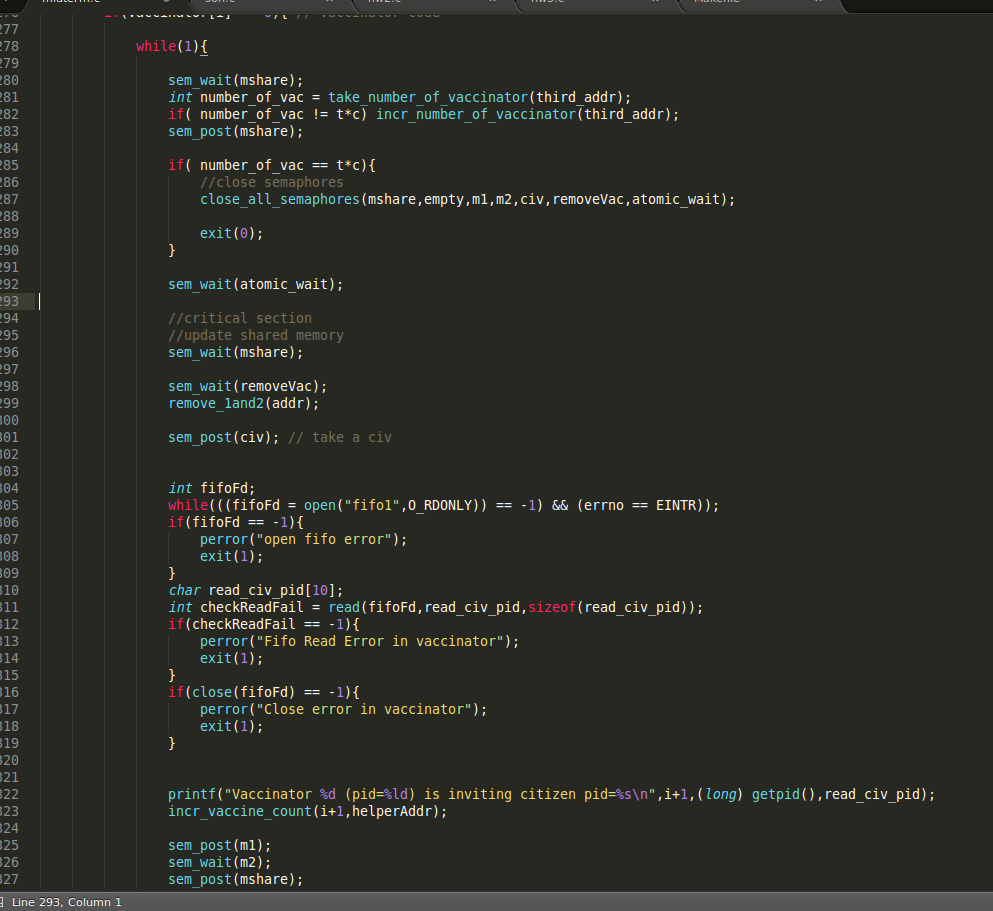
\includegraphics[scale=0.4]{vaccinator.png}
\caption{The vaccinator process code}
\label{fig:nurse}
\end{figure}

\newpage

\begin{figure}[h!]
\centering
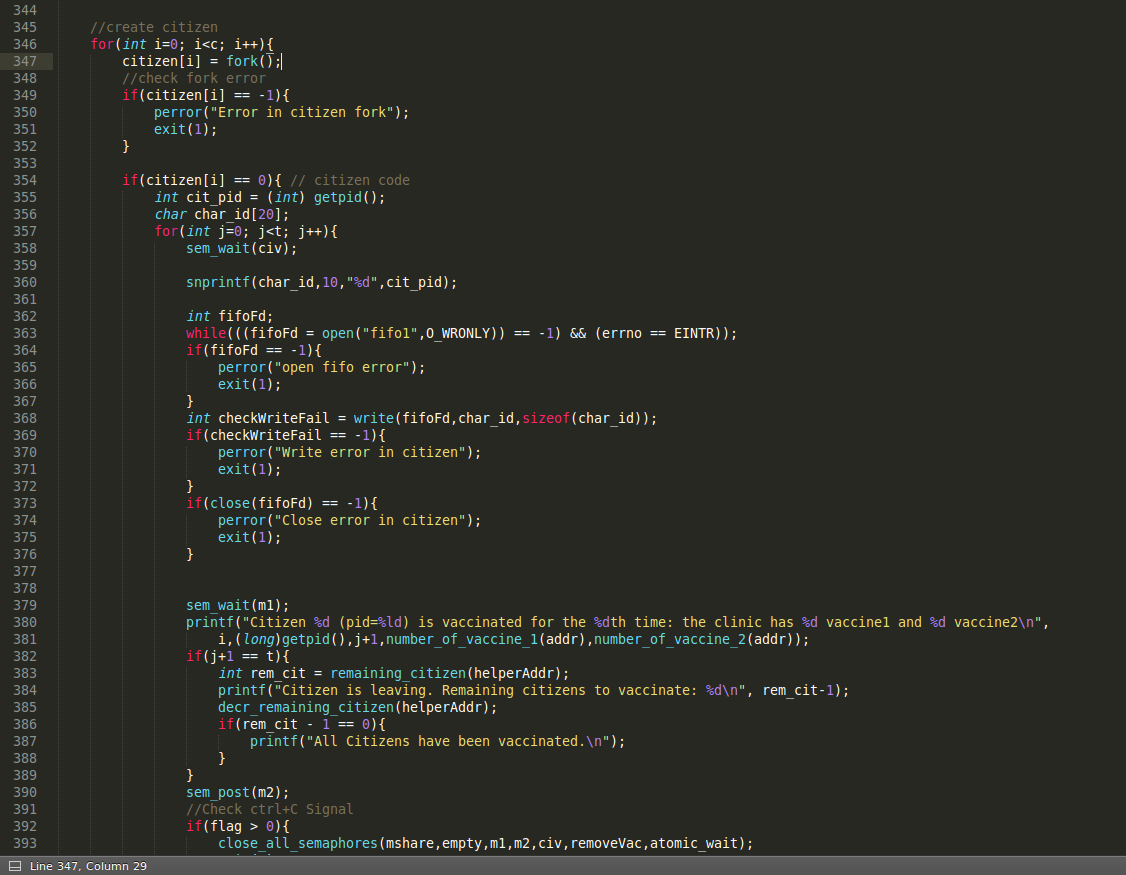
\includegraphics[scale=0.4]{citizen.png}
\caption{The citizen process code}
\label{fig:citizen}
\end{figure}

Citizen wait in semwait(civ) for a vaccinator aweke them. Then awakened citizen use fifo that we opened in vaccinator and send its own pid to vaccinator. Then wait m1 semaphore wait for vaccinator print invite message then citizen can continue and print its message. Also thirs shared memory used in citizen for printing remaining citizens information.
\\
\textbf{Ctrl C signal} \\
In case of ctrl c signal I use a flag in signal handler. Child processes check this flag in their code. If a signal arrived at least one of the child terminated because of the ctrl c signal. Then parent will kill all children and print a signal catch message and terminate after closing all shared memory and semaphores.
\\
\newpage
In my program design, Vaccinator block another invite before a citizen take its vaccine. So in my output, After every vaccinator invite message there is citizen vaccinated message.\\
\textbf{Output example} \\
./program -n 10 -v 4 -c 6 -b 40 -t 6 -i inputFile
\begin{figure}[h!]
\centering
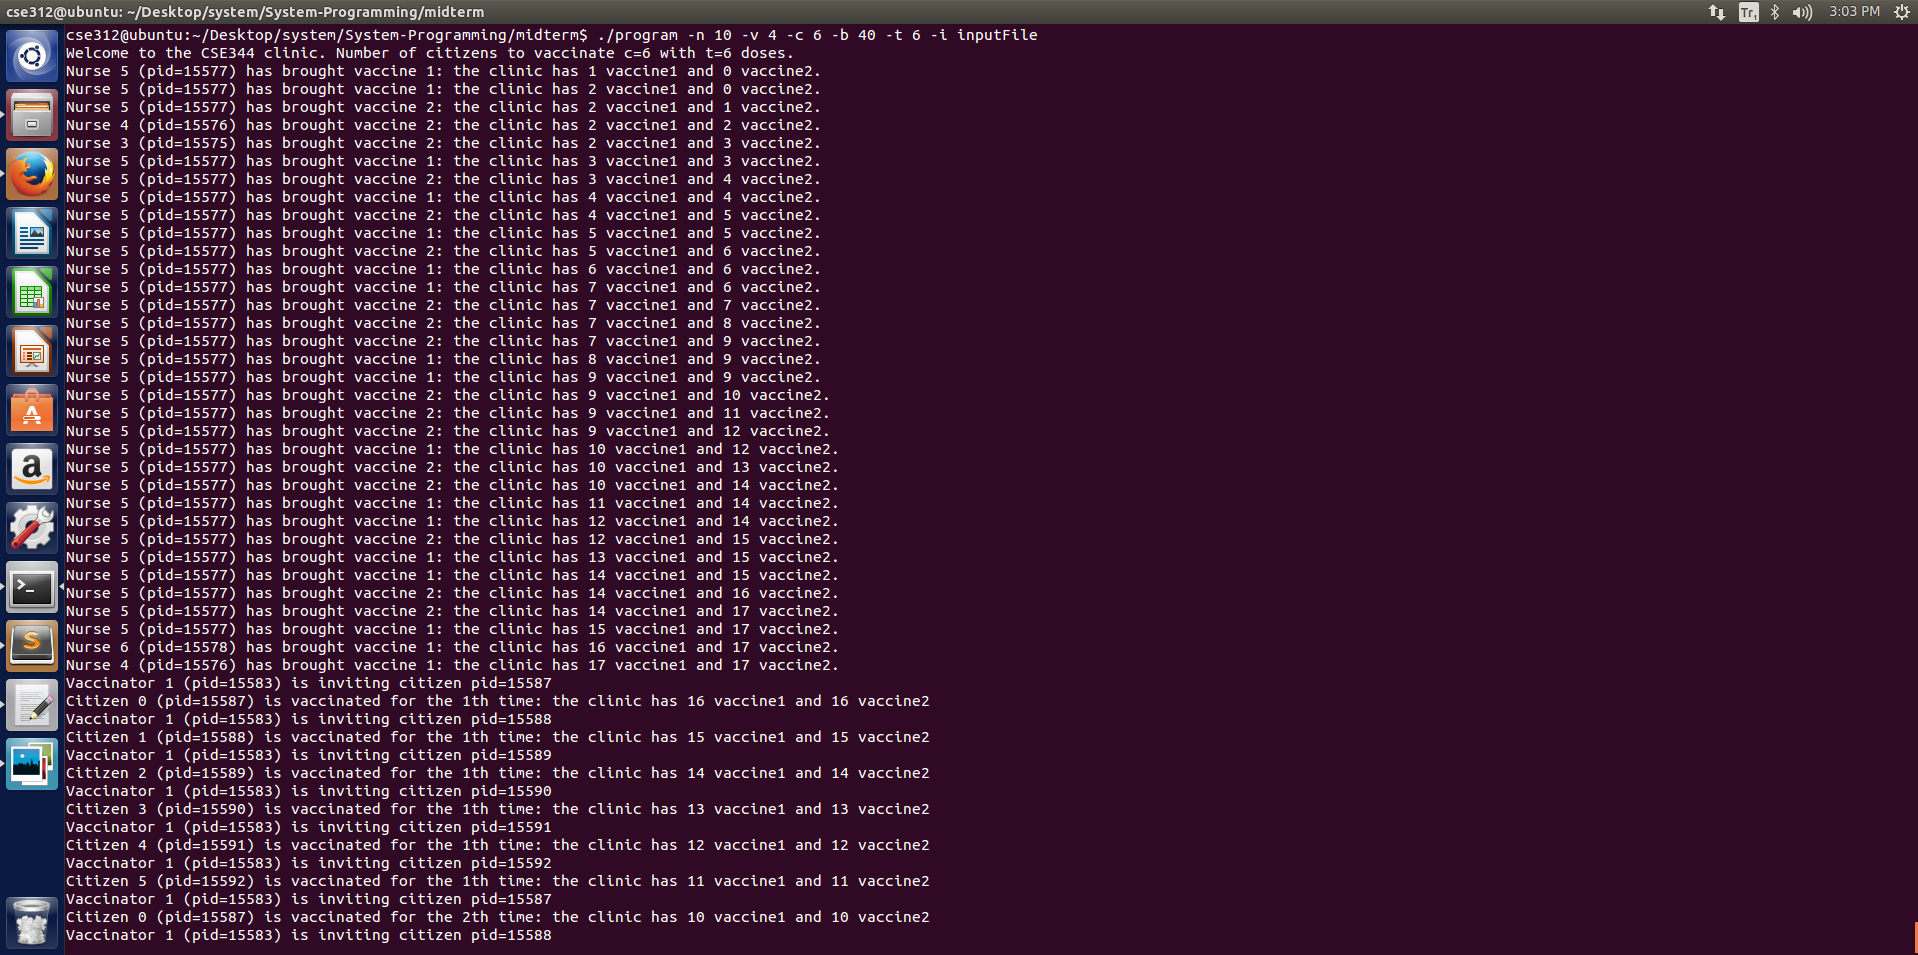
\includegraphics[scale=0.3]{run1.png}
\caption{Running start}
\label{fig:citizen}
\end{figure}
\\
\begin{figure}[h!]
\centering
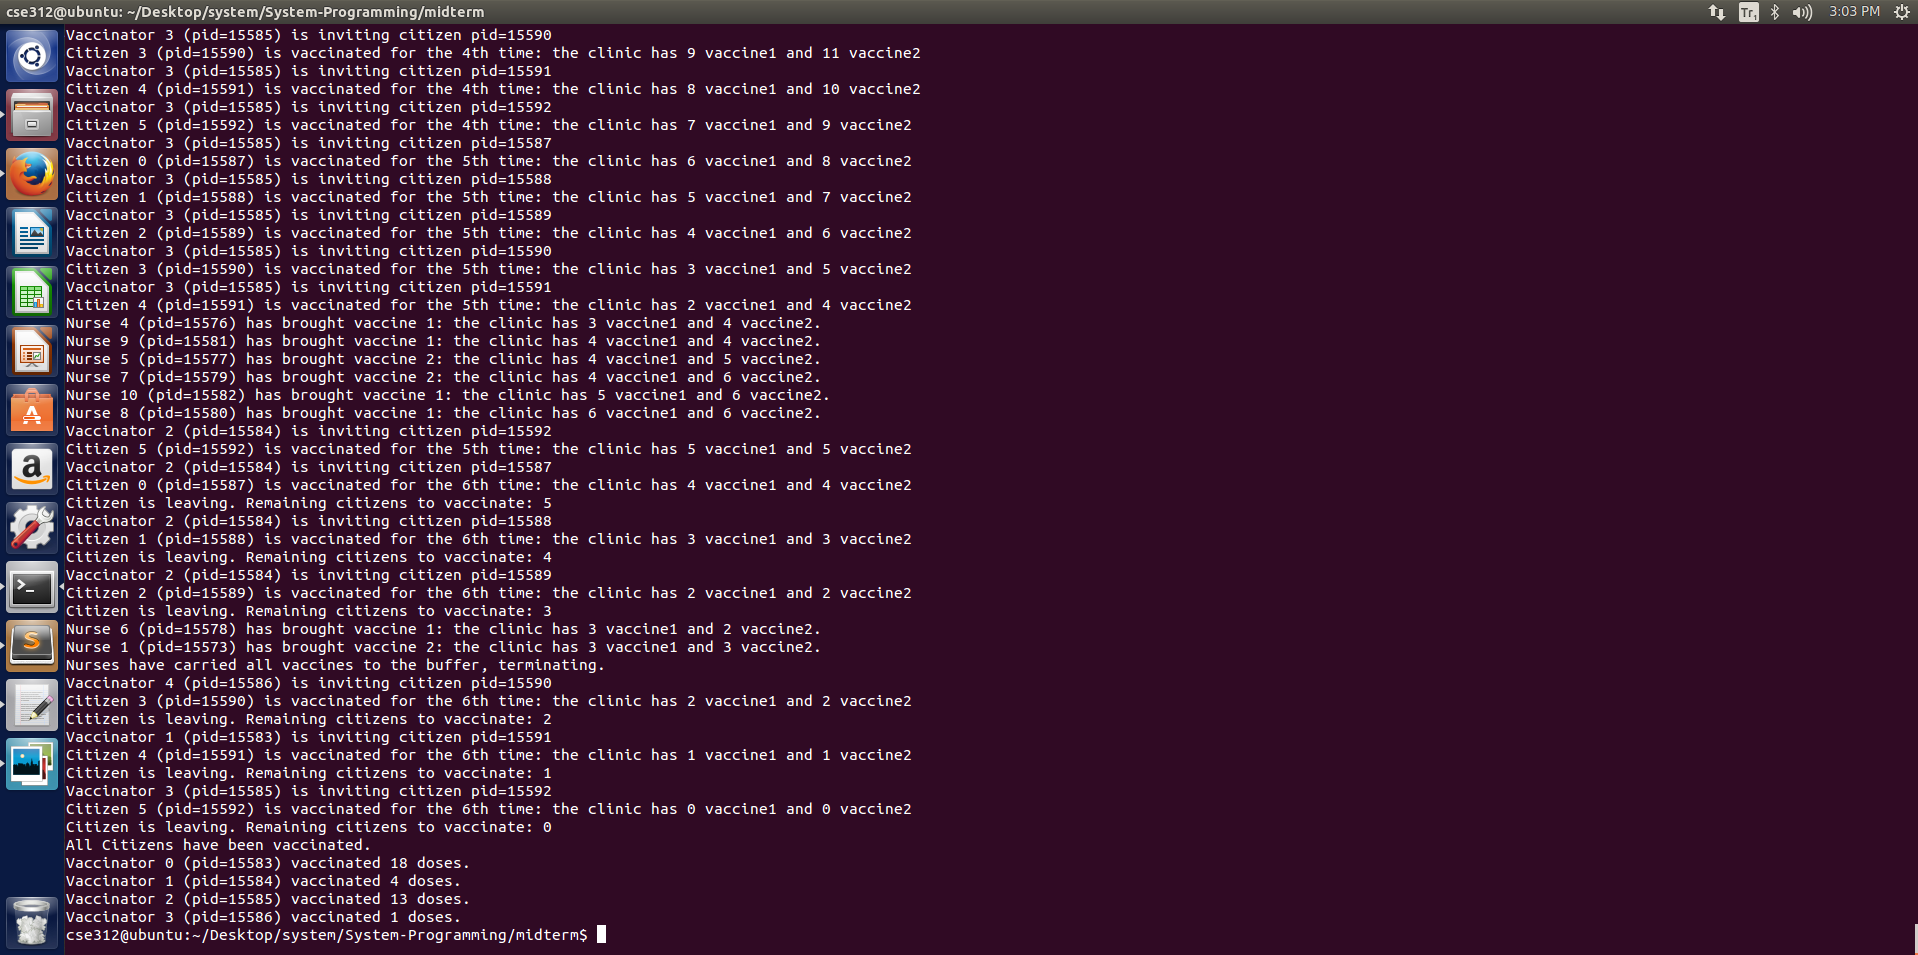
\includegraphics[scale=0.3]{run2.png}
\caption{Running end}
\label{fig:citizen}
\end{figure}
\\ 
Valgrind example shows no memory leak.
\begin{figure}[h!]
\centering
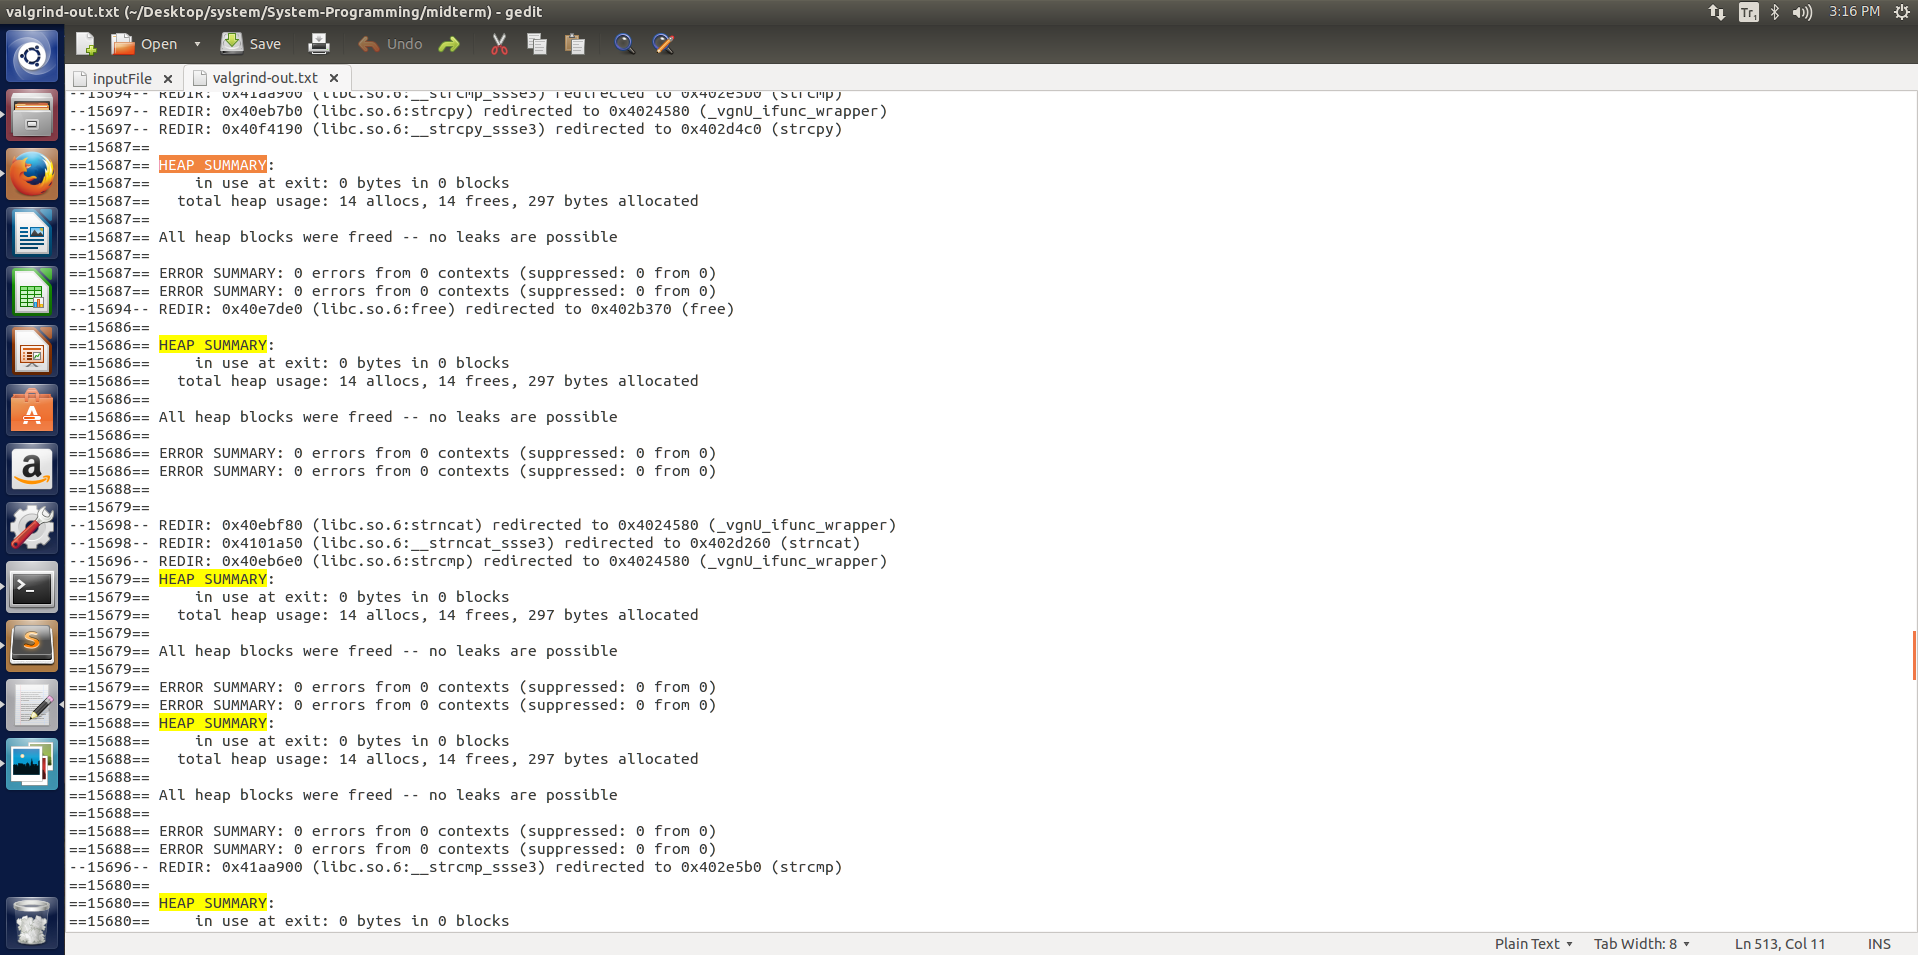
\includegraphics[scale=0.3]{valgrindHeap.png}
\caption{Valgrind output memory leak}
\label{fig:citizen}
\end{figure}

\end{document}
